%%
%% This is file `mcmthesis-demo.tex',
%% generated with the docstrip utility.
%%
%% The original source files were:
%%
%% mcmthesis.dtx  (with options: `demo')
%%
%% -----------------------------------
%%
%% This is a generated file.
%%
%% Copyright (C)
%%     2010 -- 2015 by Zhaoli Wang
%%     2014 -- 2016 by Liam Huang
%%     2016 -- 2018 by Xuehan Sun
%%
%% This work may be distributed and/or modified under the
%% conditions of the LaTeX Project Public License, either version 1.3
%% of this license or (at your option) any later version.
%%
%% This work has the LPPL maintenance status `maintained'.
%%
%% The Current Maintainer of this work is Xuehan Sun.
%%
\documentclass{mcmthesis}
\mcmsetup{CTeX = false,   % 使用 CTeX 套装时,设置为 true
        tcn = 011, problem = B,
        sheet = true, titleinsheet = true, keywordsinsheet = true,
        titlepage = true}
\usepackage{amsmath, amssymb}
\usepackage{mathrsfs}
\usepackage{palatino}
\usepackage{mwe}
\usepackage{graphicx}
\usepackage{subfig}
\usepackage{subcaption}
\usepackage{float}
\usepackage{multirow}
\usepackage{indentfirst}
\usepackage{gensymb}
\usepackage[ruled,lined,commentsnumbered]{algorithm2e}
\usepackage{geometry}
\usepackage{pdfpages}
\usepackage{array}
\usepackage{verbatim}
\usepackage{algorithm}
\geometry{left=2cm,right=2cm,top=2cm,bottom=2cm} %%页边距
\begin{document}
\linespread{0.6} %%行间距
\setlength{\parskip}{0.5\baselineskip} %%段间距
\title{DroneGo: Humanitarian In the Sky to Offer Quick and Adequate Response to Disaster-stricken Regions}

\date{\today}
	\begin{abstract}

	
		\begin{keywords}
		
		\end{keywords}
	\end{abstract}

\maketitle

\tableofcontents

\newpage

\section{Introduction}

\subsection{Problem Background}

Catastrophic disasters never stops disturbing people's peaceful life, causing many fatalities and huge economic losses. An important method to minimize the effects of terrible disasters is to offer quick and adequate response during or after disasters occur. 

In 2017, Hurricane Maria, the worst hurricane on record to strike the United territory of Puerto Rico, caused severe damages and large casualties, the image of which is presented in Figure \ref{Fig:hurr}(a). The electrical power and cell service outages lasted for months, and many highways and roads across the island were damaged severely. Demands for medical supplies and other medical facilities increased drastically. However, it was barely possible for ground vehicles to access the disaster-stricken region, since roadways were heavily damaged by widespread flood, as shown in Figure \ref{Fig:hurr}(b).

\begin{figure}[htbp]
    \begin{minipage}{0.45\linewidth}
      \centerline{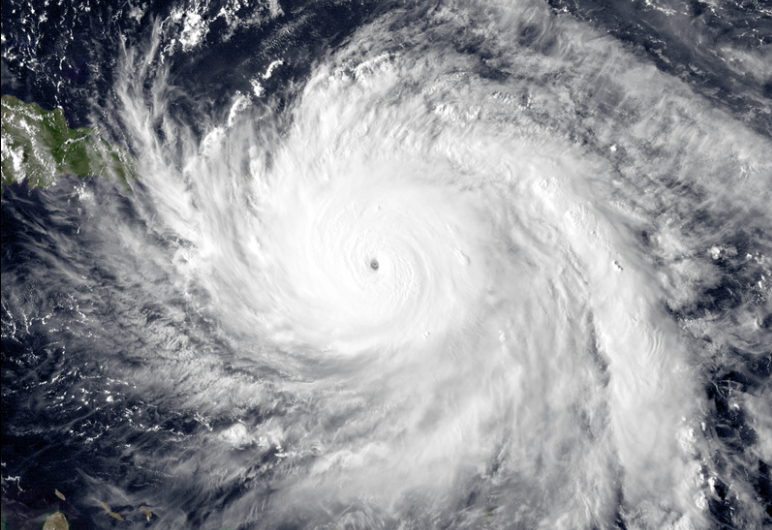
\includegraphics[height = 5.0cm,width=8cm]{figures/hurricanemaria.png}}
      \caption*{(a) Hurricane Maria near peak intensity, moving north towards Puerto Rico, on September 19, 2017.}
    \end{minipage}
    \hspace{0.5in}
    \begin{minipage}{0.45\linewidth}
      \centerline{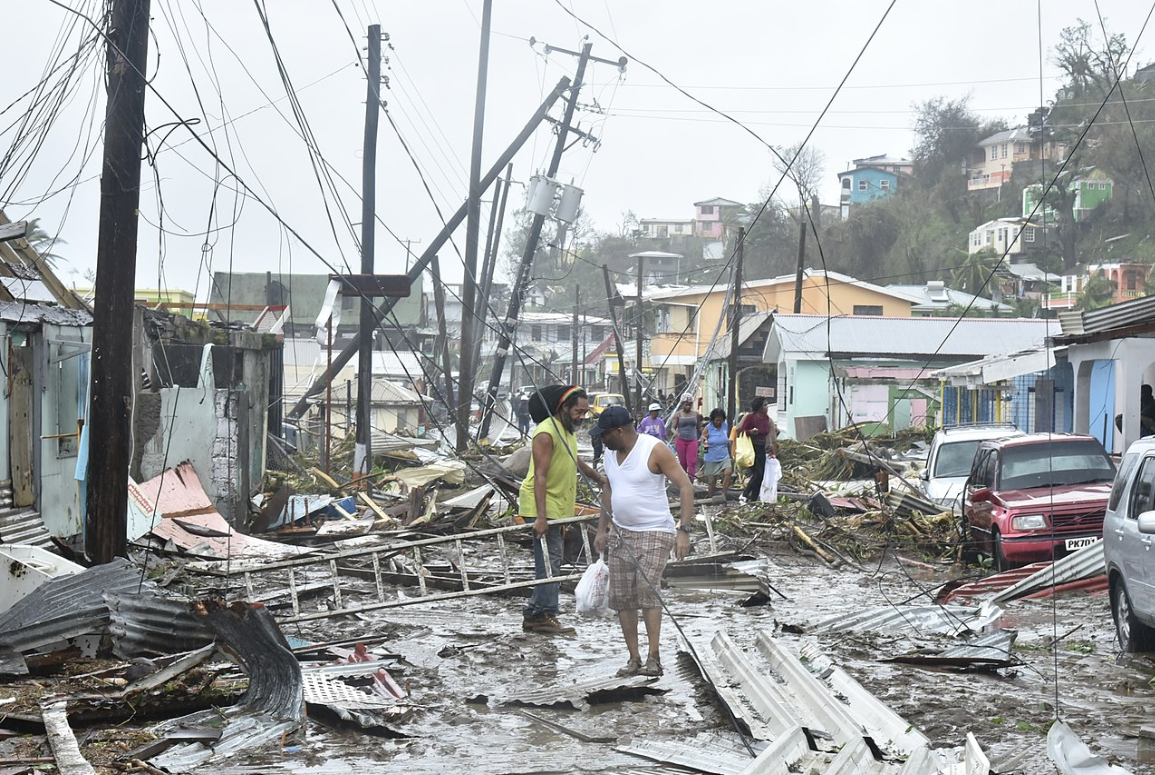
\includegraphics[height=4.9
      cm,width=8cm]{figures/hurricanedamage.png}}
      \caption*{(b) A road is littered with structural debris, damaged vegetation and downed power poles and lines, due to floodings cause by Hurricane Maria}
    \end{minipage}
    \caption{Severe Damages Caused by Hurricane Maria\cite{HurricaneMariaWiki}}
    \label{Fig:hurr}
\end{figure}

Unmanned Aerial Vehicles(UAV), though, is able to perform humanitarian tasks fully and timely, thanks to its means of shipping and fast speed. Its picture is shown in Figure \ref{Fig:uavd}. Therefore, a Non-governmental organization(NGO)-HELP,INC.-aims to promote its disaster response capabilities by applying rotor wing drones to deliver pre-packaged medical supplies and provide high-resolution aerial video reconnaissance, simultaneously or separately. This augments local medical assistance organizations to a great extent.

\begin{figure}[htbp]
    \centering
    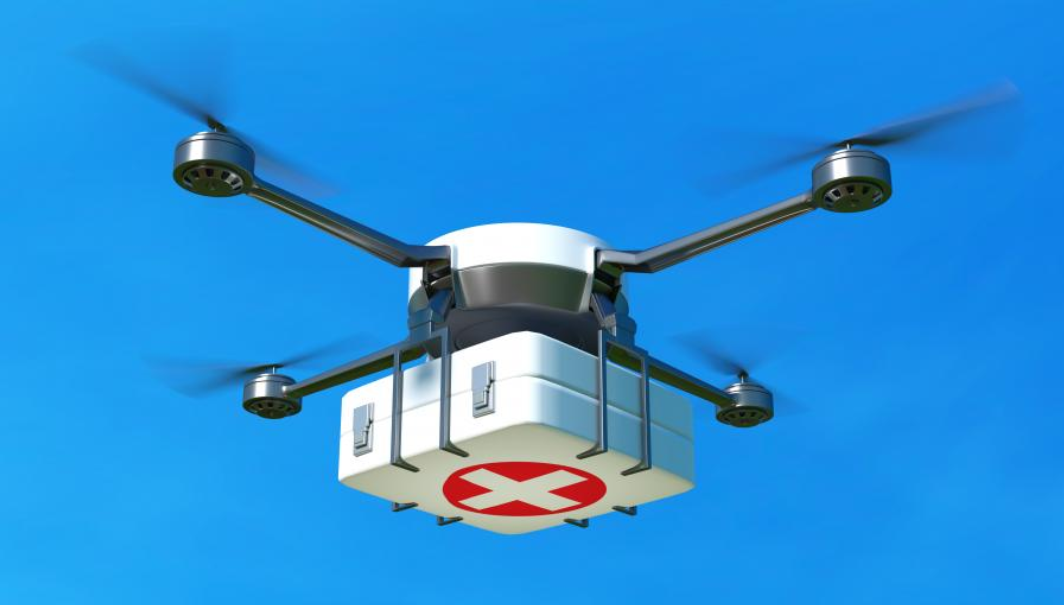
\includegraphics[height=5cm,width=8cm]{figures/uavdisasterrelief.png}
    \caption{UAV for Disaster Relief Purpose}
    \label{Fig:uavd}
\end{figure}

In order to save limited resources and equipment, the location of response system container is confined, the total $C_i$ and type of drone cargo bay as well as drone fleets are restricted, and the system has to go to great lengths to accomplish the two tasks, adequate medical supply delivery and video reconnaissance. 

\subsection{Our work}


















\section{Assumptions}
Our model makes the following assumptions:











\section{Nomenclature}










\section{Statement of our Model}\label{Sec:stat}

\subsection{Container Internal Placement Model}



\subsubsection{The Possible Layout of Container}



\subsubsection{3D Packaging Judgement}

\text{在砌墙时,人们一般会先放置一块参考砖,并以参考砖的高度作为基准,规定每个物体的高度都不能超过参考砖的高度,当物体不能放入时,则提高参考砖的高度。受此思想的启发,我们在三维装箱过程中,在水平和垂直方向上同时引入"参考"来引导装填过程。我们使用了记录可放置点来查找装填位置。该方法与其他方法的不同之处在于并不需要装填结果满足一定的结构,这使得装填过程非常灵活,并且通过引入水平参考线和垂直参考线来引导装填过程。}

\paragraph{Inspiration:}When building up a wall, people generally place a brick for reference in the first place. Then, people set the height of the brick for reference as a benchmark, and stipulate the height of each object placed-inside less than the benchmark. The benchmark can be heightened, only when no object can be placed inside.

\paragraph{Operation:}During our three-dimension packing process, similar reference line is introduced in horizontal and vertical directions to guide \textbf{the container-loading course}. 




We abstract the drone and drone cargo bay into a box.

Suppose we have boxes series $\{b_1,b_2,\dots,b_n\}$. At the beginning, the 1st box $b_1$ can be put at $(0,0,0)$. If we put it, $b_2$ has three available points $(l_1,0,0),(0,w_1,0),(0,0,h_1)$. Suppose 2ed box chooses $(l_1,0,0)$, we delete $(l_1,0,0)$ and add $(l_1+l_2,0,0),(l_1,w_2,0),(l_1,0,h_2)$ to the set of available points.

\begin{figure}
    \begin{minipage}{0.48\linewidth}
    \centerline{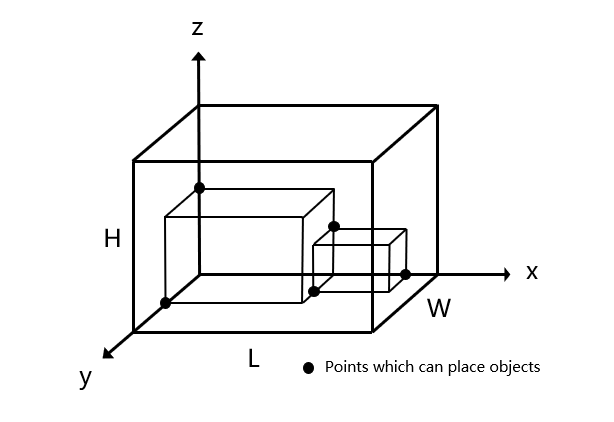
\includegraphics[width=9.0cm]{figures/availablepoints.png}}
    \centerline{(a) Available Points}
    \end{minipage}
    \begin{minipage}{0.48\linewidth}
    \centerline{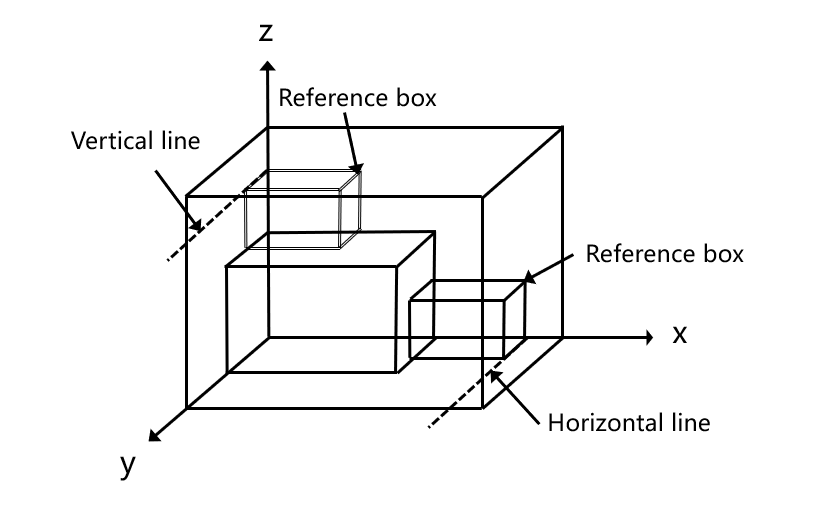
\includegraphics[width=10.0cm]{figures/hvline.png}}
    \centerline{(b) Horizontal and Vertical Line}
    \end{minipage}
    \caption{Caption}
    \label{Fig:packing}
\end{figure}

As for reference line, we select the reference line $L_z$ on the $Z$ axis and the reference line $L_x$ on the $x$ axis. Our strategy is: we consider the box in order,


The algorithm complexity is $O(n^3)$. So in order to simplify the problem, we consider that the boxes can not rotate horizontally.


\subsubsection{Generation of the Layout of Container}





\subsection{Container Location Selection Model}


\subsubsection{Location Selection}


\subsubsection{Energy Consumption}

Total \textbf{flight time} of a single drone varies, as \textbf{the weight of cargo} should be taken into account. After investigating kinds of UAVs for similar purposes and researching relevant factors that influence flight time, we generate a formula of UAV's flight time $(T_i,i\in\{B,C,D,E,F,G\})$ in Equation \eqref{Equa:ener}~\cite{DroneFlightTime}.

\begin{equation}\label{Equa:ener}
    T_i = \frac{C_i \times D_i \times V_i}{\bar{A_i} \times P_i}
\end{equation}

where:
\begin{itemize}
\item $T_i$ stands for the total Flight Time of each drone;
\item $C_i$ is the Battery Capacity of each drone;
\item $D_i$ is the Battery Discharge of each drone that is allowed for during the flight, which is typically a default value ;
\item $\bar{A_i}$ is the All Up Weight of every drone;
\item $P_i$ is P is the Power required to lift one kilogram of equipment.
\end{itemize}

Based on the given \emph{Flight Time No Cargo} data in $Attachment\,2$, and rated parameters of batteries, $A_i$ or \textbf{net weight} of each UAV can be obtained. We use the parameter $m_i$ to denote net weight of each UAV. As soon as the UAV is loaded with packaged cargo, $A_i$ equals to the sum of $m_i$ and payload carried. In this way, Equation \ref{Equa:ener} turns to Equation \ref{Equa:time} as follows:

\begin{equation}\label{Equa:time}
    T^{'} = \frac{C_i \times D_i \times V_i \times T_i \times P_i}{C_i \times D_i \times V_i + m_i \times T_i \times P_i}
\end{equation}

In Way-back Route Selection Model, each UAV only has two status, namely \textbf{cargo occupied} or \textbf{cargo vacant}. Therefore, there are two kinds of total flight time, which represents max delivery time possible$(T_{i1})$ and max return time possible $(T_{i2})$. $T_{i1}$ and $T_{i2}$ can be generated from Equation \ref{Equa:ener} and Equation \ref{Equa:time}. However, the outright battery capacity is a limited number, so there exists a restricting Equation \ref{Equa:rest}.

\begin{equation}\label{Equa:rest}
\frac{t_{i1}}{T_{i1}}+\frac{t_{i2}}{T_{i2}} = 1
\end{equation}


\subsubsection{Drone Payload Packing Configuration}




\subsection{Route Selection Model}














\subsubsection{Road Coverage}

\subsubsection{Route Planning}



\section{Implementation}

\subsection{Data}












\section{Model Analysis}

\subsection{Sensitivity Analysis}


\subsection{Strengths and Weaknesses}

\subsubsection{Strengths}

\subsubsection{Weaknesses}





\section{Conclusions}



\section{Memo to the HELP.INC CEO}





\bibliographystyle{IEEEtran}
\bibliography{newrefs}

\newpage

\begin{appendices}







\section{Implemented Algorithms and Codes}
\subsection{3D Packaging Judgement}
\begin{algorithm}  
  \caption{3D Packaging Judgement}  
  \KwIn{$B=\{b_1,b_2,\dots,b_n\}$}  
  \KwOut{True $or$ False}  
  $I=\{(0,0,0)\}, L_z = L_x = 0,count=0$\;
  \For{$i=1;i \le n;i ++$}  
  {  
    $flag = false$\;
    \For{$(x,y,z)\in I$}
    {
        \If{$b_i$ can be put into position $(x,y,z)$ and $x+ l_i\leq L_x, z+ h_i\leq L_z$}
        {
            $flag$= True,Break\;
        }
        \If{$flag$= False}
        {
            \If{$L_x=0$ or $L_x=L$}
            {
                \If{$b_i$ can be put into position $(0,0,L_z)$}
                {
                    $x=0,y=0,z=L_z,flag=$True$,L_z=L_z+h_i,L_x=l_i$\;
                }
                \ElseIf{$L_z<H$}
                {
                    $L_z=H,L_x=L,i=i-1$\;
                }
            }
            \Else
            {
                \For{$(x,y,z)\in I$ and $x=L_x,y=0$}
                {
                    \If{$b_i$ can be put into position $(0,0,L_z)$ and $z+h_i\leq L_z$}
                    {
                        $flag$=True$,L_x=L_x+l_i,$Break\;
                    }
                }
                \If{$flag=$False}
                {
                    L_x=L,i=i-1\;
                }
            }
            
        }
        \If{$flag$=True}
        {
            Put $b_i$ into position $(x,y,z)$, $I=I/{(x,y,z)}$, move $b_i$ along the X, Y, Z axis coordinate reduction direction and get $(x',y',z')$, $I=I\cup \{(x'+l_i,y',z'),(x',y'+w_i,z'),(x',y',z'+h_i)\}$,$count++$ 
        }
    }
  }
\Return $count==n$\;  
\end{algorithm}  



\end{appendices}
\end{document}


